\section{Electromagnetic Concepts}
\subsection{Maxwell's Equations}
\begin{itemize}
    \itemsep0pt
    \item Maxwell Equations in differential form (with excitations):
        \begin{align*}
            &\nabla \times \vec{H} = j\omega\epsilon\vec{E} + \vec{J},\
            &\nabla \cdot \left(\epsilon\vec{E}\right) = \rho,\\
            &\nabla \times \vec{E} = -j\omega\mu\vec{H} - \vec{M},\
            &\nabla \cdot \left(\mu\vec{H}\right) = \rho_m,\\
            &\left[\vec{H} = \dfrac{1}{\mu} \nabla\times\vec{A}\right],\
            &\left[\vec{E} = -\dfrac{1}{\epsilon} \nabla\times\vec{F}\right]\\
            &\vec{A}:\text{magn. vector potential},\\
            &\vec{F}:\text{elek. vector potential}\\
        \end{align*}
        \textbf{Boundary conditions}\\
        \begin{minipage}{.25\paperheight}
            \centering
            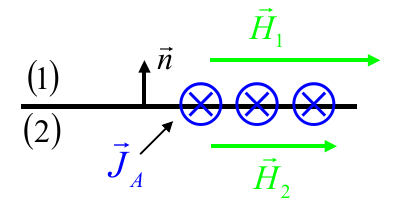
\includegraphics[width=\textwidth]{content/aawp/pictures/EH_field_boundary_condition.png}
            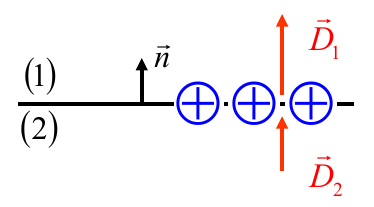
\includegraphics[width=\textwidth]{content/aawp/pictures/BD_density_boundary_condition.png}
        \end{minipage}
        \begin{align*}
            &\vec{n} \times \left(\vec{H_1} - \vec{H_2}\right) =\
            \begin{cases} 0 & \quad \text{standard}\\ \vec{J_a} & \quad \text{surface current density} \end{cases}\\
            &\vec{n} \times \left(\vec{E_1} - \vec{E_2}\right) =\
            \begin{cases} 0 & \quad \text{standard}\\ \vec{-M_a} & \quad \text{surface current density} \end{cases}\\
        \end{align*}
        \begin{align*}
            &\vec{n} \cdot \left(\vec{D_1} - \vec{D_2}\right) =\
            \begin{cases} 0 & \quad \text{standard}\\ \vec{\rho}_A & \quad \text{surface charge density} \end{cases}\\
            &\vec{n} \cdot \left(\vec{B_1} - \vec{B_2}\right) =\
            \begin{cases} 0 & \quad \text{standard}\\ \vec{\rho}_{mA} & \quad \text{surface charge density} \end{cases}\\
        \end{align*}
\end{itemize}
\subsection{Green's Functions}
\begin{itemize}
    \itemsep0pt
    \item A Green's function is the field distribution of a \textit{Dirac Delta source distribution} (e.g. field of a Hertzian dipole).
    \item Charaterizes solution similar to how the behaviour of an LTI system is charaterized by an \textit{impulse response}.
    \item For simple solution domains (eg. free space) Green's functions are known in analytical form.
    \item Fields of arbitrary source distribution as \textit{integral over the source distribution}:
        %\(\vec{E} = \iiint \dyade{G}(\vec{r}, \vec{r^\prime}) \cdot \vec{J}(\vec{r^\prime}) \mathrm{d}v^\prime\)
        \begin{align*}
            \vec{A} &= \iiint\limits_V \dyade{G}_J^A(\vec{r},\vec{r}^\prime) \cdot \vec{J}(\vec{r}^\prime)\:\mathrm{d}v^\prime,\\
            \vec{F} &= \iiint\limits_V \dyade{G}_M^F(\vec{r},\vec{r}^\prime) \cdot \vec{M}(\vec{r}^\prime)\:\mathrm{d}v^\prime\\
        \end{align*}
    \item Free space EM-fields that are \textbf{excited by electric currents:}\\
        \begin{align*}
            &\dyade{G}^E_J(\vec{r},\vec{r}^\prime) = -j\omega\mu\left[\left(\dyade{I} + \dfrac{1}{k^2}\nabla\nabla\right) \dfrac{\mathrm{e}^{-jk\:|\vec{r} - \vec{r}^\prime|}}{4\pi|\vec{r} - \vec{r}^\prime|}\right]\\
            &\dyade{G}^H_J(\vec{r},\vec{r}^\prime) = \nabla\;\dfrac{\mathrm{e}^{-jk\:|\vec{r} - \vec{r}^\prime|}}{4\pi|\vec{r} - \vec{r}^\prime|} \times \dyade{I}\\
            &\vec{E_1} = -j\omega \left[\dyade{I} + \dfrac{1}{k^2}\nabla\nabla\right] \cdot \vec{A},\;\
            \vec{H_1} = \dfrac{1}{\mu} \nabla \times \vec{A}
        \end{align*}
    \item Free space EM-fields that are \textbf{excited by magnetic currents:}\\
        \begin{align*}
            &\dyade{G}^E_M(\vec{r},\vec{r}^\prime) = -\nabla\;\dfrac{\mathrm{e}^{-jk\:|\vec{r} - \vec{r}^\prime|}}{4\pi|\vec{r} - \vec{r}^\prime|} \times \dyade{I}\\
            &\dyade{G}^H_M(\vec{r},\vec{r}^\prime) = -j\omega\epsilon\left[\left(\dyade{I} + \dfrac{1}{k^2}\nabla\nabla\right) \dfrac{\mathrm{e}^{-jk\:|\vec{r} - \vec{r}^\prime|}}{4\pi|\vec{r} - \vec{r}^\prime|}\right]\\
            &\vec{E_2} = -\dfrac{1}{\epsilon} \nabla \times \vec{F},\;\
            \vec{H_2} = -j\omega \left[\dyade{I} + \dfrac{1}{k^2}\nabla\nabla\right] \cdot \vec{F}
        \end{align*}
    \item Total fields in homogenous (free) space:
        \begin{align*}
            &\vec{E}(\vec{r}) = \vec{E}_1 + \vec{E}_2\\
            &\vec{H}(\vec{r}) = \vec{H}_1 + \vec{H}_2\\
        \end{align*}
\end{itemize}

\subsection{Radiation from Electromagnetic Sources}
\begin{itemize}
    \itemsep0pt
    \item Assuming homogenous (e.g. free) space:
        \begin{align*}
            \vec{B} &= \nabla\times\vec{A}\\
            \vec{E} &= -j\omega\vec{A} - \nabla\phi
        \end{align*}
    \item Vector and scalar \textit{Helmholtz-Equations}:
        \begin{align*}
            \Delta \vec{A} + k^2 \vec{A} &= -\mu \vec{J}\\
            \Delta \phi + k^2 \phi &= \dfrac{\nabla\cdot\vec{J}}{j\omega\epsilon} = -\dfrac{\rho}{\epsilon}
        \end{align*}
\end{itemize}

\subsection{Far-Field Approxamations}
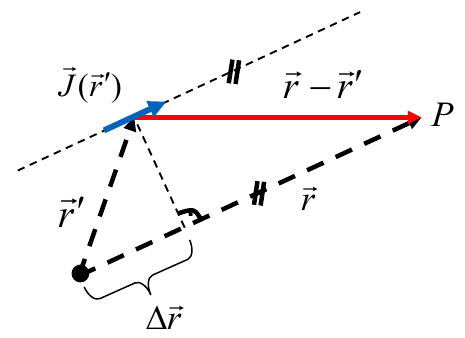
\includegraphics[width=.25\paperheight]{content/aawp/pictures/far-field_approximation.png}
\begin{itemize}
    \itemsep0pt
    \item Two different far-field approximations:\\
        \begin{itemize}
        \itemsep0pt
            \item For the dividend (amplitude): \(|\vec{r} - \vec{r}^\prime| \approx r\)
            \item For the exponent (phase):\\
            \(|\vec{r} - \vec{r}^\prime| \approx r - \Delta r = r - \dfrac{\vec{r} \cdot \vec{r}^\prime}{r}\)
        \end{itemize}
        \item Approximating in the far-field, we get:
            \begin{align*}
                &\vec{A}(\vec{r}) = \mu\dfrac{\mathrm{e}^{-jkr}}{4\pi r} \iiint\limits_V \vec{J}(\vec{r}^\prime) \mathrm{e}^{+jk\dfrac{\vec{r}^\prime \cdot \vec{r}}{r}} \:\mathrm{d}v^\prime\\
                &\vec{F}(\vec{r}) = \epsilon\dfrac{\mathrm{e}^{-jkr}}{4\pi r} \iiint\limits_V \vec{M}(\vec{r}^\prime) \mathrm{e}^{+jk\dfrac{\vec{r}^\prime \cdot \vec{r}}{r}} \:\mathrm{d}v^\prime\\
                &\nabla\times\vec{A} \approx -jk\vec{e}_r \times \vec{A}(\vec{r})\\
                &\nabla\cdot\vec{A} \approx -jk\vec{e}_r \cdot \vec{A}(\vec{r})\\
            \end{align*}
\end{itemize}
            \fbox{%
            \parbox{.3\textwidth}{%
            Spherical field components in the Far-field; \textbf{electric current source} $\vec{J}$
            \begin{align*}
                &H_{r1}=0, &E_{r1}=0,\\
                &H_{\vartheta1}=\dfrac{jk}{\mu}A_{\varphi}, &E_{\vartheta1}=-j\omega A_{\vartheta}=Z_F H_{\varphi1},\\
                &H_{\varphi1}=\dfrac{jk}{\mu}A_{\vartheta}, &E_{\varphi1}=-j\omega A_{\varphi}=-Z_F H_{\vartheta1}\\
            \end{align*}\vspace{-7mm}
                    }}
            \fbox{%
            \parbox{.3\textwidth}{%
            Spherical field components in the Far-field; \textbf{magnetic current source} $\vec{M}$:
            \begin{align*}
                &E_{r2}=0, &H_{r2}=0,\\
                &E_{\vartheta2}=-\dfrac{jk}{\epsilon}F_{\varphi}=Z_F H_{\varphi2}, &H_{\vartheta2}=-j\omega F_{\vartheta},\\
                &E_{\varphi2}=\dfrac{jk}{\epsilon}F_{\vartheta}=-Z_F H_{\vartheta2}, &E_{\varphi2}=-j\omega F_{\varphi}\\
            \end{align*}\vspace{-7mm}
                    }}


\subsection{Image Theory}
\begin{center}
    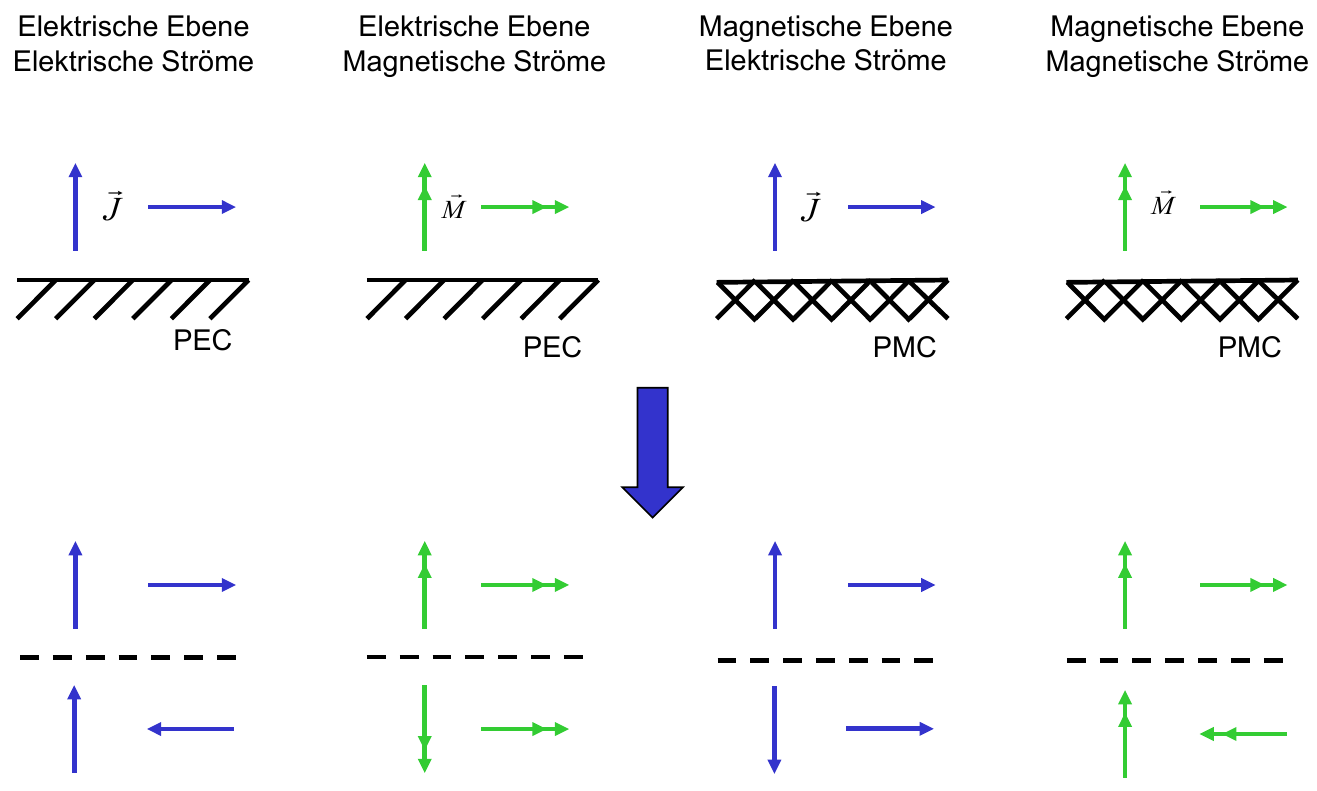
\includegraphics[width=.29\textwidth]{content/aawp/pictures/aawp_image_theory.png}
\end{center}

\subsection{Hertzian and Fitzgerald Dipoles}
\begin{itemize}
    \itemsep0pt
    \item Hertzian Dipole:
        \begin{itemize}
            \itemsep0pt
            \item Excitation for derivation of Green's function:\\
                \(\vec{J} = I_a \vec{l}_e \delta(\vec{r} - \vec{r}^\prime)\)
            \item Characteristic: \(|C(\vartheta)| = \left|\sin(\vartheta)\right|\)
            \item Radiation Resistance: \(\dfrac{2}{3} \pi Z_F \left(\dfrac{l_e}{\lambda}\right)^2 = 80 \pi^2 \Omega \left(\dfrac{l_e}{\lambda}\right)^2\)
        \end{itemize}
    \item Fitzgerald Dipole:
        \begin{itemize}
            \itemsep0pt
            \item Excitation:\\
                \(\vec{M} = I_m \vec{\Delta} \delta(\vec{r} - \vec{r}^\prime) = j\omega\mu I A \delta(\vec{r} - \vec{r}^\prime)\)
        \end{itemize}
\end{itemize}

\subsection{Reciprocity Theorem}
\begin{align*}
    &\text{\parbox{3cm}{General form of reciprocity theorem:}} &\iiint\limits_V\left(\vec{E}_1 \cdot \vec{J}_2 - \vec{H}_1 \cdot \vec{M}_2\right)\mathrm{d}v\\
    & &= \iiint\limits_V\left(\vec{E}_2 \cdot \vec{J}_1 - \vec{H}_2 \cdot \vec{M}_1\right)\mathrm{d}v,\\
    &\text{\parbox{3cm}{Form for two-port model:}} &\dfrac{U_{10}}{I_2} = Z_{12} = \dfrac{U_{20}}{I_1} = Z_{21}
\end{align*}

\subsection{Huygen's Principal}
\begin{align*}
    &\text{Mathematical form of Huygen's Principal:}\\
    \vec{E}(\vec{r})
    &= \iiint\limits_{V_b} \left[\
    \dyade{G}^E_J(\vec{r},\vec{r}^\prime)\cdot\vec{J}(\vec{r}^\prime)
    + \dyade{G}^E_M(\vec{r},\vec{r}^\prime)\cdot\vec{M}(\vec{r}^\prime) \right] \mathrm{d}v^\prime\\
    &+ \oiint\limits_{A(V_b)}\
    \left[ \dyade{G}^E_J(\vec{r},\vec{r}^\prime)\cdot\vec{J}_A(\vec{r}^\prime)
    + \dyade{G}^E_M(\vec{r},\vec{r}^\prime)\cdot\vec{M}_A(\vec{r}^\prime) \right] \mathrm{d}a^\prime,\\
    &\text{Tang. elec. current: }\vec{J}_A(\vec{r}^\prime) = \vec{n} \times \vec{H}(\vec{r}^\prime),\\
    &\text{Tang. magn. current: }\vec{M}_A(\vec{r}^\prime) = -\vec{n} \times \vec{E}(\vec{r}^\prime)
\end{align*}
\begin{enumerate}
    \itemsep-1pt
    \item Calculate $\vec{J}_A$ and $\vec{M}_A$.
    \item Enclose the entire AUT in a Huygen's surface.
    \item Keeping $\vec{J}_A$ and $\vec{M}_A$, we can formally replace the enclosed antenna's material (no net fields) with whatever we please $\implies$ free space.
    \item Determine the AUT characteristics using the (free space) \textit{Green's functions}.
\end{enumerate}

